\documentclass[12pt,preprint]{aastex}
\usepackage{lsst}
\usepackage{xspace}
\usepackage[english]{babel}
\usepackage[utf8x]{inputenc}
\usepackage{amsmath}
\usepackage{graphicx}
\usepackage{longtable}
\usepackage{hyperref}
\usepackage{comment}

\newcommand{\Alert}{\code{Alert}\xspace}
\newcommand{\Alerts}{\code{Alerts}\xspace}
\newcommand{\DIASource}{\code{DIASource}\xspace}
\newcommand{\DIASources}{\code{DIASources}\xspace}
\newcommand{\DIAObject}{\code{DIAObject}\xspace}
\newcommand{\DIAObjects}{\code{DIAObjects}\xspace}
\newcommand{\DB}{{Level 1 database}\xspace}
\newcommand{\DR}{{Level 2 database}\xspace}
\newcommand{\Object}{\code{Object}\xspace}
\newcommand{\Objects}{\code{Objects}\xspace}
\newcommand{\Source}{\code{Source}\xspace}
\newcommand{\Sources}{\code{Sources}\xspace}
\newcommand{\ForcedSource}{\code{ForcedSource}\xspace}
\newcommand{\ForcedSources}{\code{ForcedSources}\xspace}
\newcommand{\CoaddSource}{\code{CoaddSource}\xspace}
\newcommand{\CoaddSources}{\code{CoaddSources}\xspace}
\newcommand{\SSObject}{\code{SSObject}\xspace}
\newcommand{\SSObjects}{\code{SSObjects}\xspace}
\newcommand{\VOEvent}{\code{VOEvent}\xspace}
\newcommand{\VOEvents}{\code{VOEvents}\xspace}
\newcommand{\transSNR}{5\xspace}

\begin{document}
\title{Large Synoptic Survey Telescope as a Near-Earth Object Discovery Machine}

\author{R. Lynne Jones$^1$, Colin Slater$^1$, Joachim Moeyens$^1$, 
Lori Allen$^2$, Mario Juri\'{c}$^1$,  \and \v{Z}eljko Ivezi\'{c} $^1$}

\affil{
$^1$University of Washington, \\
$^2$National Optical Astronomy Observatory}


\begin{abstract}
We discuss the ability of LSST to contribute to Near-Earth Objects (NEO) discoveries and
Congressional Brown mandate to NASA. The two main issues addressed here are robustness 
of the LSST strategy for discovering NEOs using nightly pairs of observations, and the 
expected cumulative completeness for potentially hazardous asteroids (PHAs) with 
visual absolute magnitudes $H<22$.  We argue that the observing and data processing 
strategies chosen by LSST are robust, and would yield a completeness of about 70\% with 
the current LSST baseline survey. We describe a number of modifications of the LSST baseline 
survey which could potentially yield the completeness of 90\% for $H<22$ PHAs. 
\end{abstract}

\keywords{}

\section{Introduction}

XXX This is so totally work in progress. ZI push-ed it just as a backup... XXX


Main parts:
\begin{itemize}
\item NEO impacts as concern; the Brown mandate, NASA panels,
  introduce LSST 
\item LSST defaults and claimed performance in older publications
\item informal concerns by the community, GMS paper
\item study by the JPL team, technical support from LSST (assuming
  baseline cadence)
\item exploration of baseline cadence modifications designed to boost
    NEO completeness 
\item Outline of this paper
\end{itemize} 


The small-body populations in the Solar System, such as asteroids, trans-Neptunian objects (TNOs) 
and comets, are remnants of its early assembly. Collisions in the main asteroid belt between Mars and 
Jupiter still occur, and occasionally eject objects on orbits that may place them on a collision course 
with Earth. About 20\% of this near-Earth Object (NEO) population, the so-called potentially hazardous 
asteroids (PHAs), are in orbits that pass sufficiently close to Earth's orbit, to within 0.05 AU, that 
perturbations with time scales of a century can lead to intersections and the possibility of collision. 
In December 2005, the U.S. Congress directed\footnote{For details see http://neo.jpl.nasa.gov/neo/report2007.html} 
NASA to implement a NEO survey that would catalog 90\% of NEOs with diameters larger than 140 meters 
by 2020 (the George E. Brown, Jr. mandate). For a compendium of information about NEOs and PHAs 
and an up-to-date summary of discovery progress, see NASA's NEO webpage\footnote{http://neo.jpl.nasa.gov/neo/}. 

The completeness level set by Congressional mandate can be fulfilled with a 10-meter-class ground-based
telescope equipped with a multi-gigapixel camera, and a sophisticated and robust data processing system. 
The Large Synoptic Survey Telescope (LSST), currently being constructed, is such a system (for a concise
system description, science drivers and other information, see \citep{LSSToverview}). Early simulations of 
LSST performance presented by \cite{IvezicNEO2007} showed that the 10-year baseline cadence would 
result in 75\% completeness for PHAs greater than 140 m (more precisely, for PHAs with $H<22$; see 
\S~XX for further discussion). They also suggested that with additional optimization of the observing cadence, 
LSST could achieve 90\% completeness. Such optimization was discussed by \cite{LSSToverview} who
reported that, to reach 90\% completeness, about 15\% of observing time would have to be dedicated to NEOs
and the survey would have to run for 12 years.  
%% From the overview paper: 
%% - the LSST baseline cadence provides orbits for 82% of PHAs larger than 140 meters after 10 years of operations
%% - 84% completeness with minor changes to the cadence (5% of time for NEO-optimized observations)
%% - 90% completeness with major changes to the cadence (15% of time for NEO-optimized observations and 12 years)
The latest LSST simulation results, presented in \cite{JJI2016}, yielded a completeness of $\sim$72\% for
PHAs with $H<22$ using the current 10-year baseline survey. The minor difference compared to older
studies is attributable to the differences in simulated NEO populations and other modeling details. 


\cite{JPLstudy} described a new study, related to this work. Their preliminary results indicate a completeness
of $\sim$65\% for NEOs with $H<22$. The difference compared to \cite{JJI2016} result (72\%) is due 
to XXX (true?): PHA vs. NEO, possible slope of the size distribution. 


We're going to evaluate moving object detection capabilities with
LSST, comparing performance of our current prototype pipelines with 
the required performance during operations.  The two main goals are
to demonstrate that i) MOPS can cope with false detection in image differences,
and that ii) the NEO detection performance of the LSST baseline cadence can be
further boosted by adequate modifications 


From JPL paper -- which gives a concise summary of the main simulation aspects. 

The LSST baseline survey cadence relies primarily on single night pairs of detections, 
with roughly 30 minutes between the elements of a detection pair. These pairs form 
what are known in MOPS parlance as tracklets, and sets of tracklets are linked across 
multiple nights to form tracks, which can then be sent to the final step, which is orbit 
determination. The strategy of using pairs is an aggressive and potentially fragile
approach, but theoretically represents the most productive NEO search with the minimum 
impact on other LSST science drivers. An alternative to visit each field three times per 
night to form tracklets from triplets of detections may prove more robust, but likely 
with a penalty of reduced performance. One of our study objectives is to understand the
tradeoffs between these two approaches.

The two major questions to be addressed by our study can be informally stated as 
``Will MOPS work?'' and ``If MOPS works what fraction of NEOs will LSST discover?''. 

Main problems:
\begin{enumerate}
\item Linking large number of detections in the presence of false positives (false detections due to problems 
with image differencing software). 
\item Adequacy of data, including image depth, sky coverage and cadence, to reach the required 
completeness level. 
\end{enumerate} 

Therefore, the main analysis components to check are: 
\begin{enumerate}
\item The performance of image differencing, with emphasis on the rate and properties of 
   false detections 
\item Linking large number of detections in the presence of false positives 
\item Observing cadence simulations coupled with NEO population models to forecast 
        discovery rates 
\end{enumerate} 



\cite[hereafter GMS]{GMS2016} reported different NEO completeness levels than
published by the LSST team in 2007 and 2014 . There are three main 
reasons why the GMS results differ:
\begin{enumerate}
\item GMS used a different realization of the LSST baseline survey
\item GMS used different synthetic NEO populations to evaluate completeness
\item GMS {\it redefined} the completeness limit from the commonly
  used $H<22$ criterion to an albedo-dependent value of $H$ limit (which
  attempts to directly model the $D>140$ m size cut)
\end{enumerate}

Regarding the last point, GMS found that the completeness drops by 5\%
when $H<22$ criterion is replaced by $D>140$ m criterion. Regarding 
the first point, GMS results can be more meaningfully compared to an LSST
study by \cite{JJI2016}, who used the same simulated cadence. After accounting for 
the $H<22$ vs. $D>140$ m methodological difference of 5\%, GMS obtained a 
completeness of 67\% using 3 pairs in 12 nights (for simulated cadence {\it enigma\_1189}), while Jones et al. 
study obtained $\sim$73\% using 3 pairs in 15 nights (for simulated cadence {\it minion\_1016}, which is 
statistically very similar to {\it enigma\_1189}). This difference 
of $\sim$5\% is attributable to the differences in simulated NEO
populations and other modeling details. In summary, GMS find the NEO
completeness in the range $\sim$60\% to $\sim$70\% for the LSST
baseline cadence. The variation is due to different NEO populations,
different NEO detection criteria, and other specifics. When accounting 
for different choices of simulation parameters, their results are
consistent with the results published by the LSST team. 

But: how much higher can the completeness be pushed with cadence
modifications optimized for NEOs? 

In Observing Strategy white paper: fig. 3.4 gives 73.4\% for PHAs with 
$H<22$ and {\it minion\_1016}, using 3 pairs in 15 nights. 


\begin{enumerate} 
\item Control and quantify the rate of (false positive) detections
\item Software (and computational capacity) capable of inter-night linking of detections given the expected rates
\item Quantify the discovery yields (and their robustness) under those assumptions
\end{enumerate} 


The leading systematic effects in completeness estimates are: 
\begin{enumerate}
\item NEO vs. PHA difference (the completeness is about $\sim$5\% higher for PHAs than for NEOs) 
\item Different sample definitions: $H<22$ vs. $D>140$m (as shown by \citep{GMS2016}, completeness
           increases by $\sim$5\% when $H$-based criterion is used) 
\item Orbital parameter distribution for the simulated asteroid population (e.g. the Bottke model
             vs. the Granvik model; varying populations contribute completeness uncertainty of a few percent) 
\item Variations of ``discovery window'' (e.g., X visit pairs in N nights: changing N from 15 to 30 with X=3 increases
          completeness by 3\%; changing X from 3 to 4 with N=15 decreases completeness by 6\%; 
          additionally, if the nominal detection threshold is changed from the signal-to-noise ratio of 5 or greater  
          to 4 or greater, the completeness is boosted by 2-3\%). 
\item Variations of the nominal detection threshold (if the detection threshold is changed from the 
          signal-to-noise ratio of 5 or greater to 4 or greater, the completeness is boosted by 2-3\%). 
\item Sensitivity to details in sky coverage and cadence (e.g. nightly pairs of visits vs. quads of visits;
          requiring quads instead of pairs of visits decreases completeness by 30\% using baseline cadence; 
          about half of that loss can be recovered using cadence simulations that request four visits per night) 
\item Uncertainties when predicting effective image depth (system throughput, variation of the detection efficiency
          with the signal-to-noise ratio, treatment of trailing losses); for a survey that has a completeness above 60\%, 
          each additional one magnitude of depth for a given survey cadence increases the completeness by another 10\%.
\item Uncertainties when predicting apparent flux (albedo distribution, phase effects, photometric variability 
          due to non-spherical shapes, color distributions); assuming an uncertainty of 0.2 mag in the effective 
          limiting magnitude, the corresponding  systematic uncertainty in completeness is about 2\%.)
\item The slope of the asteroid size distribution (current measurement uncertainty of this parameter 
          corresponds to a systematic uncertainty in completeness of about 2\%.)
\item The impact of known objects (assuming that 43\% objects would be discovered by the start of
          LSST survey, \citep{GMS2016} boosted the final PHA completeness for LSST baseline survey by 11\%). 
\end{enumerate} 

Given these systematic effects, a comparison of different simulation results (both of the same system,
and of different systems, especially those operating at different wavelengths) has to be undertaken
with due care. It is unlikely that a meaningful quantitative comparison can be pushed beyond a level
of a few percent (and perhaps as much as 10\%). In practice, the completeness of a given operating survey
is best estimated using the object re-discovery rate. 


From Mario's talk to NASA:

LSST will detect variability (motion and flux variability) by
differencing each incoming image against a deep template.
Sources will be detected at an S/N=5 threshold (see Appendix A). 

We expect on average about 1,000 per sq. deg. astrophysical, real,
detections, including up to about 500 asteroids per sq. deg on the 
Ecliptic (for scale, the LSST field of view is about 10 sq. deg., with 
about 20 4kx4k CCDs per sq. deg.)

We also expect a false-positive detections due to random
fluctuations in the background at a level of about 200 per
sq. deg. (all at the faint end).  XXX check Colin's report 

However, historically surveys have reported factors of 10 to 500 times
more (depending on the survey; see \citep{denneau13};
\citep{goldstein15} ). 
Those additional false positive
detections are due to systematic effects: 
\begin{itemize} 
\item Camera and telescope artifacts
\item Imperfect image subtractions
\item Cosmic rays
\end{itemize} 

For a ``menagerie'' of artifacts (with amusing names such as 
{\it chocolate chip cookies, frisbee, piano, arrowhead, UFO}), from
Pan-STARRS, see Fig.~17 in \cite{denneau13}. 


``Many of the false detections are easily explained as internal
reflections, ghosts, or other well-understood image artifacts,...''


Learning from PS1 Experience: PanSTARRS was a first generation
experiment. Over the past decade, subsequent surveys (including LSST) 
have learned tremendously from the PS1 experience. There are surveys 
running today which have largely solved the key problems that PS1 has encountered.
These are recent developments driven largely by extragalactic and
transient science cases. They are not yet well known beyond those
communities and reporting on those developments is additional
motivation for this paper. 
 
Major improvements to hardware include CCDs with significantly fewer 
artifacts (e.g. DECam, see below; LSST) and optical systems designed to
minimize ghosting and internal reflections (e.g. LSST). 

Improvements to the software include advanced image differencing
pipelines (e.g., PTFIDE for the Palomar Transient Factory and the
Zwicky Transient Facility) and various machine learning classifiers
for filtering false positives (see below). 

DECam: \cite{goldstein15} 

The Dark Energy Survey (DES) is an optical/near-infrared survey that
aims to probe the dynamics of the expansion of the universe and the
growth of large scale structure by imaging 5,000 sq. deg. of the
southern sky. It is technologically very similar to LSST with
\begin{itemize}
\item 520 Mpix camera, 62 mosaicked chips (deep depleted devices)
\item 3 sq.deg. field of view, same filter bands as LSST
\item Single-exposure depths comparable to LSST
\item Includes a supernova search program which employs image
differencing methods analogous to LSST’s  and detects objects at the 
same effective signal-to-noise ratio as LSST (S/N=5)
\end{itemize} 

The false positives in DECam data are morphologically much simpler
(compare Fig.~1 in \citep{goldstein15} to Fig.~17 in \citep{denneau13})
than those in Pan-STARRS, and thus are much more amenable to automated 
screening using machine learning methods. Using a Random Forest 
classifier, \cite{goldstein15} cleaned their sample from having a 
raw false detection rate of 13:1 to a filtered rate of 1:3. This performance
is already within the acceptable range for LSST performance goals. 


{\bf Need to refer to section by Colin.} 

LSST will use two methods to detect moving objects
\begin{enumerate}
\item Detecting trailed motion on the sky:  objects trailed by more
  than 2 PSF widths (corresponding to motion faster than about 1
  deg/day) will be easily detectable as trailed.  Two trailed
  detections within 30--60 minutes in a single night will be
  sufficient to identify an object as an NEO candidate,
\item Inter-night linking of pairs: this technique will recover
  objects moving too slow enough to be measurably elongated in 
  a single exposure. 
\end{enumerate} 

MOPS: Given the expected false-positive rates demonstrated by
\cite{goldstein15} and in Colin's  section, LSST MOPS linking will
be possible. This has already been shown by the PanSTARRS project 
with simulations performed for the PS4 system\footnote{PanSTARRS 
PS1 experience does not contradict this conclusion. In addition to 
hardware issues, PS1 was only 1/4 of the assumed system (see 
\citep{denneau13} for more details). }, which is in this
respect equivalent to LSST. The robustness to unexpected false
positives is further tested with simulations performed by LSST,
as described below. 







\section{LSST Solar System Survey} 

Opening paragraph  (lift text from overview and Lynne's IAU paper) 

Possible subsections here or below:

- Concepts for discovering moving objects

- Outline for simulations (see Chesley) 




\subsection{Brief Overview of LSST} 
%\subsection{Brief Overview of LSST} 

LSST will be a large, wide-field ground-based optical telescope system
designed to obtain multiple images covering the sky that is visible
from Cerro Pach\'{o}n in Northern Chile. The current baseline design,
with an 8.4m (6.7m effective) primary mirror, a 9.6 deg$^2$ field of
view, and a 3.2 Gigapixel camera, will allow about 10,000 square
degrees of sky to be covered every night, with typical 5$\sigma$ depth 
for point sources of $r\sim24.5$ (AB). The system is designed to yield 
high image quality (the median delivered seeing in the $r$ band of 
about 0.8 arcsec) as well as superb astrometric  and photometric 
accuracy\footnote{For detailed specifications, please see the LSST
Science Requirements Document, http://ls.st/srd}. The total survey
area will include $\sim$30,000 deg$^2$ with $\delta<+34.5^\circ$, and 
will be imaged multiple times in six bands, $ugrizy$, covering the 
wavelength range 320--1050 nm. For a more detailed, but still concise,
summary of LSST, please see 
the LSST Overview paper\footnote{arXiv:0805.2366, http://ls.st/2m9}. 

The project is scheduled to  begin the regular survey operations at
the start of next decade. About 90\% of the observing time will be
devoted to a deep-wide-fast survey mode which will uniformly observe 
a 18,000 deg$^2$ region about 1000 times (summed over all six bands) 
during the anticipated 10 years of operations, and yield a coadded map 
to $r\sim27.5$. These data will result in catalogs including about
$40$ billion stars and galaxies, that will serve the majority of the
primary science programs. The remaining 10\% of the observing time
will be allocated to special projects such as a Very Deep and Fast
time domain survey\footnote{Informally known as ``Deep Drilling Fields".}.

The LSST will be operated in fully automated survey mode. The images
acquired by the LSST Camera will be processed by LSST Data Management
software \cite{juric15} to a) detect and characterize imaged
astrophysical sources and b) detect and characterize temporal changes
in the LSST-observed universe. The results of that processing will be
reduced images, catalogs of detected objects and the measurements of 
their properties, and prompt alerts to ``events'' -- changes in
astrophysical scenery discovered by differencing incoming images
against older, deeper, images of the sky in the same direction ({\em
emplates}, see \S \ref{sec:AppA} for more details). 
 

\subsection{LSST Observing Strategy} 

XXX get text from the overview paper and Science Book 

As deployed and funded (by the U.S National Science Foundation and
Department of Energy), LSST is primarily a science-driven mission. 
Existing cadence is optimized to maximize the overall science returns
(incl. Solar System science), rather than NEO/PHA discovery
completeness (though the two goals are highly interrelated).  As designed, the survey is not optimized for rapid
discovery and follow-up of all types of moving objects\footnote{
XXX What's the purpose of this footnote? Note that LSST will enable rapid identification and follow-up of
trailed objects (within 60 seconds of discovery). If deployed with a 
planetary-defense optimized cadence, the NEO yields could be
significantly improved, and approaching the 90\% completeness level
for $H<22$.} 
Early simulations indicate 90\% is achievable for NEO-optimized
cadence. However, other science goals would be affected (including
Solar System science!).  XXX Refer to Jones et al.  (2016) 

The current baseline cadence is optimized for science returns.
It is expected to yield approximately $\sim$70\% of the extant NEO population.


\subsection{LSST  Data Management and Image Processing} 

Refer to \cite{DM2016} and Appendix A. 


%\section{Image Differencing Performance}
\section{Analysis of Image Differencing Performance \label{sec:imDiff}}

LSST will detect motion and flux variability by differencing each incoming image
against a deep template (built by combining multiple images of the same region).
Sources in difference images, called \DIASources, will be detected at a signal-to-noise
ratio (SNR) threshold of $\nu=5$. Up to about 1,000 deg$^{-2}$
astrophysical, real, detections (e.g. variable stars) are expected in LSST image differencing, including
up to about 500 deg$^{-2}$ asteroids on the Ecliptic. In addition to real detections,
there are false detections due to imaging or processing artifacts and 
false detections caused simply by statistical noise
fluctuations in the background. In a typical LSST difference image, the expected
density of false detections due to background fluctuations is about 60 deg$^{-2}$
(see below for details)---much lower than the expected rate of astrophysical
detections (see \S\ref{sec:kaiser} below). 

However, historically surveys have reported detection rates in image differencing that are much
higher, depending on the survey; see \cite{denneau13}; \cite{kessler15}; \cite{goldstein15}.
For example, Pan-STARRS1 (PS1) reported a transient detection rate as high as 8,200 deg$^{-2}$
\citep{denneau13}. For a ``menagerie'' of PS1 artifacts (with memorable names such as
{\it chocolate chip cookies, frisbee, piano, arrowhead, UFO}), see Fig.~17 in \cite{denneau13}.
They reported that ``Many of the false detections are easily explained as internal reflections,
ghosts, or other well-understood image artifacts, ...''. As discussed in \S\ref{sec:tracklets},
such a high false detection rate is at the limit of what could be handled even
with the substantial computing power planned for LSST.

Fortunately, Pan-STARRS1 was only a first-generation experiment and, over the past decade,
subsequent surveys have learned tremendously from the PS1 experience. There are surveys
running today, such as Dark Energy Survey, which have largely solved the key problems that
PS1 has encountered. Major improvements to hardware include CCDs with significantly fewer
artifacts (e.g. DECam, see below; LSST) and optical systems designed to minimize ghosting
and internal reflections (e.g. LSST). Improvements to the software include advanced image
differencing pipelines (e.g., PTFIDE for the Palomar Transient Factory and the Zwicky Transient
Facility) and various machine-learning classifiers for filtering false detections. For example,
\cite{goldstein15} used a Random Forest classifier with the Dark Energy Survey data
and cleaned their sample of transient detections from a raw false:true detection
rate ratio of 13:1 to a filtered rate of 1:3. The resulting false detections are
morphologically much simpler; for example, compare
Fig.~1 in \cite{goldstein15} to Fig.~17 in \cite{denneau13}.

Here we summarize an analysis of image differencing performance based on DECam
data and difference images produced and processed using prototype LSST
software \citep{DMTN-006}. This analysis demonstrates that the false
detection rate anticipated for LSST (without using any machine-learning classifiers for
filtering false positives) is significantly below the threshold for
successful deployment of MOPS, as will be discussed in \S\ref{sec:mops}.



\subsection{LSST Image Differencing Pipeline and Data Processing}

The LSST prototype image differencing and analysis code largely derives from the
HOTPANTS package \citep{becker15}, and was used for surveys such as SuperMACHO
\citep{becker05} and ESSENCE \citep{miknaitis07}. While this software is
functional as-is, it is expected that the ultimate LSST pipeline will include
improved methods for handling observations at high airmass and the effects of
differential chromatic refraction due to the Earth's atmosphere. Nevertheless, in
this work we conservatively assume that the pipeline used for LSST will have the
same performance as the current code.


\subsection{False Detections due to Background Fluctuations \label{sec:kaiser}}

Some false detections are expected simply due to background fluctuations, even
at a high SNR threshhold. The number of
such detections, as a function of the threshold SNR, the number of pixels and
seeing, can be computed using the statistics of Gaussian random fields.
For an image with a Gaussian background noise, convolved with a Gaussian point
spread function (PSF) with width $\sigma_g$ (in pixels), the number of peaks, $N$, above a
given SNR threshold, $\nu$, is given by (N. Kaiser, priv. comm.)
\begin{equation}
N(>\nu)  = \frac{n_{row}*n_{col}}{2^{5/2} \, \pi^{3/2} \, \sigma_g^2} \, \nu \, e^{-\nu^2 /2}
\label{eq-theory}
\end{equation}
where $n_{row}$ and $n_{col}$ are the number of pixel rows and columns in the image.
This expression was verified empirically by LSST data management team using
image simulations\footnote{See \url{https://github.com/lsst/W13report}}.
For 4k by 4k LSST sensors the pixel size is 0.2 arcsec, and for a nominal seeing
of 0.85 arcsec and $\nu=5$, $N(>\nu) = 59$ deg$^{-2}$.

It is generally not well appreciated just how steep is the dependence of $N(>\nu)$
on $\nu$ due to the exponential term. Changing the threshold from 5 to 5.5
decreases the expected rate by a factor of 12, and the rate increases by a factor
of 9.7 when the threshold is changed from 5 to 4.5. In practice, an empirical estimate
of the background noise is used when computing the SNR for each detected source.
When this estimate is incorrect, e.g. due to reasons discussed below, then the
implied detection threshold is wrong, too. For example, if the noise is underestimated
by only 10\%, the computed SNR will be too large by 10\%, and the adopted
threshold $\nu=5$ will actually correspond to $\nu=4.5$ -- and thus the
sample will include 9.7 times as many false detections due to background
fluctuations! Hence, the noise in difference images has to be estimated to
high accuracy.


\subsubsection{The Impact and Treatment of Correlated Noise}

When the LSST pipeline convolves the science image to match the PSF of the template
image, the per-pixel variance in the image is reduced, and at the same
time correlations between neighboring pixels are introduced. This violates the
assumption made by standard image processing algorithms that each pixel is an
independent draw from a Poisson distribution. The per-pixel noise reduction is
reflected in the variance plane that accompanies each exposure during
processing, but the covariance between pixels is not tracked.
The significance of detections and the uncertainties on source measurements is
then estimated based on this incomplete information provided by the variance
plane, leading to a biased detection threshold.

The magnitude of this effect can be large---using only the per-pixel variance
measurements can result in underestimating the true noise on PSF-size scales by
20\% or more. A detection threshold of $\nu=5$ thus actually corresponds to
$\nu=4$, and it is easy to see using eq.~\ref{eq-theory} that this error results
in an increase in the number of false positives by a factor of $\sim$70!

A histogram of the number of sources detected in difference images, as a function
of SNR computed using forced photometry measurements, is shown in the right panel
of Figure~\ref{fig:snr_comparison}. The blue line shows the expected counts given
by eq.~\ref{eq-theory}, in good agreement with data. When the SNR is estimated
incorrectly due to correlated noise (left panel), the distribution clearly ramps
up at a much higher SNR value and results in numerous false detections that are
mis-classified as $>5 \sigma$ detections.

Tracking the covariance caused by multiple convolutions is a planned feature for
the LSST software stack, but is not currently implemented. Previous surveys, such as
Pan-STARRS1, have used a small covariance ``pseudo-matrix'', which tracks the
covariance between a small region of neighboring pixels, and then assumed that
this relationship between pixels is constant across an image (Paul Price, priv. comm.).
This method avoids the creation of the full $N_{\rm pixels}$ by $N_{\rm pixels}$
covariance matrix, which is impractically large and mostly empty.

In the interim, for this analysis we have mitigated the problem by utilizing forced photometry of \DIASources
on individual images (that is, before convolution to match their PSFs). This
produces both flux measurements and associated uncertainties which are not
affected by covariance, enabling us to accurately set a SNR threshold
that recognizes and rejects all \DIASources with $\nu < 5$. This mitigation step
will be unnecessary once the image covariance tracking is properly implemented
in the LSST stack. Alternative solutions such as image ``decorrelation''
\citep{DMTN-021}, or the \citet{zackay} image differencing algorithm, would also
alleviate the covariance problem, and tests of these methods in the LSST pipeline are ongoing.


\begin{figure}
  \centering
  \plotone{figures/snr_comparison.pdf}
  \caption{
  Histogram of the reported SNR of sources measured in the difference images,
  using two different SNR estimates: SNR (incorrectly) estimated using the variance plane
  of the difference images (left) and SNR (correctly) estimated from forced photometry on
  the input images (right).  The blue lines indicate the expected SNR distribution
  based on Gaussian background noise. The difference between these two histograms
  illustrates the strong impact of the SNR mis-estimation. Using the correct SNR values,
  the vast majority of putative $>5 \sigma$ detections become $<5 \sigma$ detections
  and can be disregarded.
  }
  \label{fig:snr_comparison}
\end{figure}


\subsection{Testing the LSST Pipeline with DECam}

The Dark Energy Survey (DES) is an optical/near-infrared survey that aims to probe the
dynamics of the expansion of the universe and the growth of large scale structure by
imaging 5,000 sq. deg. of the southern sky. DECam, the imaging camera developed for
DES, is sufficiently similar to LSST camera to enable an informative study of false detection
rates: DECam includes 62 mosaicked deep-depletion CCDs, with a total pixel count of
520 Mpix over its 3 deg$^2$ field of view, and has a similar filter complement as LSST \citep{DECam}.

The data we use here are a subset of a DECam NEO survey (PI: L. Allen, NOAO) conducted
in the first half of 2013. The data for a given field consist of 40-second exposures separated
by about five minutes. Due to the difference in telescope aperture, these images
are about 1 mag shallower than the 30 second visits by LSST. We used data for
five different fields, each with between three and five visits for a total of 15
``science'' visits plus 5 template visits. While this section will present
statistics based on this subset of the survey's data, during the course of this
work a much larger superset of 540 visits from the same survey was also processed and
produced false detection rates broadly consistent with this initial data (on
average the 540 visits have fewer false detections by about 30\% than the small
subset.)

From the NOAO archive we obtained images that had already had instrumental
signature removal applied by the DECam Community Pipeline. Each image was
processed through the initial LSST pipeline for background subtraction, PSF
determination, source detection and measurement (collectively
termed ``processCcd'' in the LSST pipeline). For each field, we arbitrarily
selected one of the visits to serve as the ``template'' exposure, against which
the other visits in the field are differenced. Sources are then detected in the
difference image to produce \DIASources, and forced photometry performed in both
the original ``science'' and ``template'' exposures at the position of any
\DIASource.

In LSST operations, coadded prior exposures will be used
as templates for image differencing rather than single visits, which will reduce
the noise in template images. In this study, our use of single visits instead of
coadded templates implies that some moving objects or transients will appear as
negative sources in the difference images. We simply disregard these sources
since our goal is to mimic LSST operations rather than discover all possible
transients in this dataset.

%After producing difference images, we detect sources (\DIASources) and measure
%their properties. In addition, we also perform forced photometry (flux measurements
%at the positions of detected \DIASources) on individual single-epoch input images
%using the current versions of LSST pipelines \citep{juric15}.

\subsubsection{The Transient and False Positive Rates in DECam Images}

Using the $>5\sigma$ cut based on SNR estimated using forced photometry,
the average number of positive \DIASources is $\sim 1000$ deg$^{-2}$,
with some fields having as few as $500$ deg$^{-2}$. A large fraction of
these detections are the result of stars that have been poorly-subtracted and
left significant residuals in the difference image. It is a common problem for
subtracted stars to exhibit ``ringing'' with both positive and negative
excursions, and these images are no exception. Because the focus of this work
is on detecting moving objects rather than variable stars or transients, we have
not attempted to correct these subtraction artifacts. Instead, we simply exclude
difference image detections where there is significant ($>15 \sigma$) flux in both the
science and template images at the position of the \DIASource---that is, we exclude all \DIASources that
overlap with a static source (of course, some may be truly variable sources).
The area lost due to this masking is less than $1\%$ of the total sky. Again, this
is not the intended behavior of LSST during production, but instead a temporary
expedient we can use for conservatively estimating the system's performance.
One could view this step as a ``poor man's'' machine learning step.

After excluding all \DIASources associated with stationary objects, the
remaining candidate moving object detections number on average $\sim 350$
deg$^{-2}$. This sample includes asteroids, false positives, and possibly some
true astrophysical transients that are not associated with stationary objects
(gamma-ray burst afterglows, very faint variable stars with sharp light
curve maxima, etc.). To improve the estimate of the fraction of these remaining
objects that are false, we visually classified one focal plane of detections either
as obvious imaging artifacts, obvious PSF-like detections, or unidentifiable
detections. Approximately 25\% of the reported detections were clearly some
sort of uncorrected artifact (we did not pursue the cause of individual artifacts),
25\% appeared to be acceptable PSF-like features, and the remaining 50\% were
ambiguous or had too low of signal to noise to be able to classify.
Therefore, a conservative upper limit on the fraction of false detections is 75\%,
assuming the 25\% of detections which had acceptable PSF-like features were real objects,
corresponding to a rate of 263 deg$^{-2}$. Given the size of DECam pixels
(0.263 arcsec) and typical seeing of about 1.1 arcsec ($\sigma_g$ = 1.8 pix),
the expected rate due to background fluctuations is 33 deg$^{-2}$, leaving
a rate of 230 deg$^{-2}$ as ``unexplained'' false detections.

The SNR distribution of this sample is proportional to 1/SNR$^{2.5}$, which
is similar to distributions expected for astrophysical objects. This fact implies
that the sample might be dominated by true astrophysical transients and
asteroids; nevertheless, we adopt the above conservative upper limit of 75\%.


\subsubsection{Scaling DECam Results to LSST Performance}

The LSST false detection rate due to background fluctuations will be about twice
as large as for DECam because of smaller pixels and better seeing. The scaling
with pixel size and seeing for ``unexplained'' false detections is not obvious
because their cause is unknown. For example, if they are a pixel-induced effect,
their rate should be scaled up by the square of the ratio of angular pixel sizes, or
a factor of 1.72. If they are instead dominated by true astrophysical transients, 
they should not be scaled at all. Since our dataset contains an unknown 
mixture of false detections from these two types of scalings, in addition to a 
significant number of true detections, we cannot derive a precise scaling for the 
false detection rate. Instead, we adopt a {\it conservative} option by assuming
that {\it all of our detections are false} and behave like pixel-induced effects, 
which scales up the DECam rate for ``unexplained'' false positives to 396 deg$^{-2}$. 
In addition, there will be 60 deg$^{-2}$ false detections due to background fluctuations 
(eq.~\ref{eq-theory}, referenced to the median seeing of 0.85 arcsec).

The total false positive rate of $\sim450$ deg$^{-2}$ anticipated for LSST is thus
comparable to the rate of astrophysical transients. Again, this estimate of the false
positive rate is conservative and it would not be very surprising if it turns out
to be much smaller.

In addition to uncertainties mentioned above, it is hard to precisely account for 
the fact that LSST images will be about one magnitude deeper than the analyzed DECam 
images. The contribution to false detections from background fluctuations 
(60 deg$^{-2}$) should not be changed because it depends on SNR, not the
specific magnitude limit. If all remaining
false detections are due to pixel-induced effects, they are also dependent on SNR 
(i.e. counts) and not on magnitude. In this scenario, the number of false detections
would not vary even though LSST images would be deeper. If instead all remaining 
false detections are astrophysical in nature, the DECam rate (230 deg$^{-2}$) should 
{\it not} be multiplied by 1.72 for pixel-scaling, and instead should be corrected for the 
difference in image depth. Since the observed differential
\DIASource distribution scales approximately as SNR$^{-2.5}$, one magnitude of 
depth increases the sample size by a factor of about 4. More precisely, we know
that one third of the ``unexplained'' false detections are likely pixel-induced effects
(the 25\% which were clearly some uncorrected artifact above),
and no more than two thirds can be astrophysical, so the scaled rate expected
for LSST would be (1/3*1.72 + 2/3*4)*230 + 60 = 805 deg$^{-2}$, or about 
a factor of 1.8 higher than the adopted rate of $\sim450$ deg$^{-2}$. We emphasize
that this estimate corresponds to the worst case scenario that is rather unlikely
to be correct. 
  

\subsubsection{Spatially Correlated Transients}

\begin{figure}
  \centering
  \plotone{figures/stacked_tracklets.pdf}
  \caption{
   ``Stacked'' tracklets of three or more detections surrounding bright stars are shown in the left panel
  as lines. $\Delta \textrm{Dec}$ and $\Delta \textrm{RA}$ are the tracklet coordinates relative to a nearby
  bright star, such that any correlated features due to, e.g., bleed trails or
  diffraction spikes, will show a grouping of lines with similar positions and
  orientations. No such features are seen and the vast majority of
  tracklets are consistent with real moving objects (and on average aligned with
  the Ecliptic). The ``hole'' in center of the plot comes from the rejection of \DIASources
  in regions with significant flux in the template image. The right panel shows
  the position angle of the tracklets (degrees East of North), while the dashed
  vertical line indicates the angle that would be seen if the tracklets were on
  lines of constant Ecliptic latitude. Again the vast majority appear to be
  aligned with the Ecliptic.
  }
  \label{fig:stacked_tracklets}
\end{figure}

We have checked for correlations in tracklets around bright stars, which
might arise if either optical or processing artifacts exhibited some preferred
alignment. Such an alignment may create false tracklets at a rate greater than
an overdensity of uncorrelated detections would. To investigate these
correlations we generated tracklets using the current prototype version of MOPS.
For this test tracklets are required to have three or more detections (out of five visits
at each pointing) that align with velocities less than $2\deg$/day. For each
star brighter than 14th magnitude in the UCAC4 catalog \citep{UCAC4}, we
identified all tracklets within 4 arcminutes of the star, and ``stacked'' the
tracklets surrounding each star onto a single plot. The resulting tracklet
distribution can be seen in Figure~\ref{fig:stacked_tracklets}, where each black
line corresponds to a single tracklet. If, for example, there was an excess of
tracklets along CCD bleed trails from bright stars, these would appear as a set
of lines along the $\pm\Delta \textrm{RA}$ direction, or a peak at $90\deg$ or
$270\deg$ in the histogram (right panel of Figure~\ref{fig:stacked_tracklets}).
We do not see any such correlated detections after inspecting approximately
5,000 tracklets (the number in the plot is limited for legibility).

We also investigated whether \DIASources from multiple visits are correlated
in pixel coordinates, which might arise from uncorrected detector anomalies.
We analyzed a 4-visit subset of the 15 science visits used in the rest of this
work, and for each \DIASource computed the distance in pixels to any neighboring
\DIASources, even if they appeared on different visits or different fields
(similar to the 2-point correlation function). From this we identified  24
\DIASources that were located within two pixels of another \DIASource. We did
not find any correlation at larger radii. Visual inspection shows that many are
near parts of an image where a defect (such as a cosmic ray, bad column, bleed
trail, etc) had been interpolated over, though for some the cause is unclear.
The implied density of correlated \DIASources is about 2.3 deg$^{-2}$, rendering
this effect relatively unimportant.

We note that the number and implied sky density of asteroids bright enough to produce
scattered light and diffraction spike artifacts, which would appear to move at solar system
rates, is at least two orders of magnitude smaller than the sky density of asteroids down
to LSST depth on the Ecliptic. Therefore, such artifacts will be unimportant as a contributor
to false tracks.


%Paper on ``Automated Transient Identification in the Dark Energy Survey''  is \cite{goldstein15}. 


\section{Moving Object Processing Pipeline Evaluation}

Zeljko and Mario. There is a report on MOPS (LDM-156)...   XXX refer to its
results here... 

Quoting \cite{denneau13}: ``MOPS achieves $>$99:5\% efficiency in
producing orbits from a synthetic
but realistic population of asteroids whose measurements were
simulated for a Pan-STARRS4-class telescope. \dots MOPS has been
adapted successfully to the prototype Pan-STARRS1 telescope despite
differences in expected false detection rates, fill-factor loss, and
relatively sparse observing cadence compared to a hypothetical
Pan-STARRS4 telescope and survey.'' 

But we did our own analysis, too...

The LSST project has developed an enhanced prototype implementation of MOPS.
We ran simulations with LSST system and cadence, and a significantly
wider range of false positive candidate rates. 

Known limitations/caveats:
\begin{itemize}
\item Due to computational constraints at the time when the simulation
  was performed (2011), a $v < 0.5$ deg/day velocity limit was
  imposed.
\item For similar reasons, the filters were imposed on track fitting
  were not optimized, artificially reducing the yield
\item As we understand the algorithmic scalings, these will not change the
final results; nevertheless they are being actively mitigated by new
simulations which are in progress.
\end{itemize}

Simulation results: Asteroids are discoverable in the presence of significant noise.
Get more details from Lynne \& Axelrod writeup. 



\section{LSST Observing Cadence Optimization}

Lynne, new OpSim runs. 


\section{Conclusions}

{\bf Summary:} Well behaved image differencing and detection are needed for the
asteroid detection strategy adopted by LSST. This has historically
been difficult to achieve. First generation surveys have encountered
significant problems including CCD artifacts, optical system
artifacts, and software issues. Significant progress has been made
since. Contemporary surveys comparable to LSST (specifically, DES) are
already achieving false positive rates below the few:1 ratio required
for LSST MOPS (see next section). LSST image differencing will {\bf
not} be a limiting factor in its ability to discover asteroids
(including NEOs). DES experience has already demonstrated algorithms 
sufficient to meet LSST MOPS requirements.

\begin{enumerate}
\item LSST will employ the 2+2+2 MOPS discovery strategy, and detect fast-moving asteroids via trailing.
\item Existing surveys demonstrate that false positive rates required
  by LSST (approaching $\sim$1:1) are  achievable (Dark Energy Survey;  \citep{goldstein2015}).
\item PanSTARRS PS4 simulations \citep{denneau13}) as well as LSST
  simulations (Myers et al. 2011) demonstrate the ability of MOPS to perform the linkages under those conditions.
\item LSST software and observing strategy are robust to perturbations
  around assumed efficiencies; even large differences in expectation
  cause only a few percent difference in efficiency. 
\item Our simulations indicate that, if the cadence is optimized for
          NEO searches, LSST likely has the capability and capacity to reach the Brown mandate.
\end{enumerate}

Add words about consistency with \cite{GMS2016}. 

\appendix
%\section{LSST Image Processing Steps and Data Products Relevant for Asteroids} \label{sec:AppA}
\section{LSST Image Processing Steps and Data Products Relevant for Asteroids} \label{sec:AppA}

The data products produced by the LSST Data Management system are described in
LSST Document LSE-163 \citep[LSST Data Products
Definition Document,][]{LSE-163}. Here we briefly summarize parts of that
document\footnote{To ensure the continued scientific adequacy of LSST data
products, their designs and plans are periodically reviewed and updated and
thus LSE-163 is a living document -- please always consult the latest version.}
that are most relevant for discovering moving Solar System objects.

The LSST Data Management system will perform nightly analysis of difference images\footnote{A difference
image is an image produced by subtracting a science image from an appropriate
``average'' of the previously collected similar images of the same sky area, and using the
same filter.}, with the goal of detecting and characterizing astrophysical phenomena
revealed by their time-dependent nature. The detection of supernovae superimposed
on bright extended galaxies is an example of this analysis, and of course moving Solar
System objects are another example. The processing will be done on nightly/daily
basis and will result in the so-called Level 1 data products. Level 1 products will include
difference images, catalogs of sources detected in difference images (the so-called
\DIASources), static astrophysical objects\footnote{The LSST has adopted the nomenclature by
which single-epoch detections of astrophysical {\em objects} are called {\em sources}.
The reader is cautioned that this nomenclature is not universal: some surveys call
{\em detections} what LSST calls {\em sources}, and use the term {\em sources} for what
LSST calls {\em objects}.} these \DIASources are positionally associated to (the so-called \DIAObjects),
and moving Solar System objects (\SSObjects\footnote{\SSObjects used to be called
``Moving Objects'' in previous versions of the LSST Data Products baseline. The name is
potentially confusing as high-proper motion stars are moving objects as well. A more
accurate distinction is the one between objects {\em inside} and {\em outside} of the Solar
System.}). The catalogs will be entered into the Level 1 database and made available in near
real time. Notifications (``alerts'') about new \DIASources will be issued using
community-accepted standards\footnote{For example, VOEvent, see \url{http://ls.st/4tt}} within
60 seconds of observation.

The Moving Object Processing System (\code{MOPS}) pipeline combines all unassociated \DIASources into
plausible \SSObjects and estimates their orbital parameters. The three main pipeline stages
include associating new \DIASources with known \SSObjects, discovering new \SSObjects,
and orbit refinement and management. This conceptual MOPS design is illustrated in
Figure~\ref{fig:Pipe8}. Further details about the MOPS pipeline design and implementation are available
from the LSST Science Pipelines Design Document \citep{LDM-151}.
The next section briefly describes the main processing steps in nightly/daily Level 1 data processing.

\begin{figure}[!t]
    \centering
    %\vskip -2.3in
%    \hskip -0.2in
    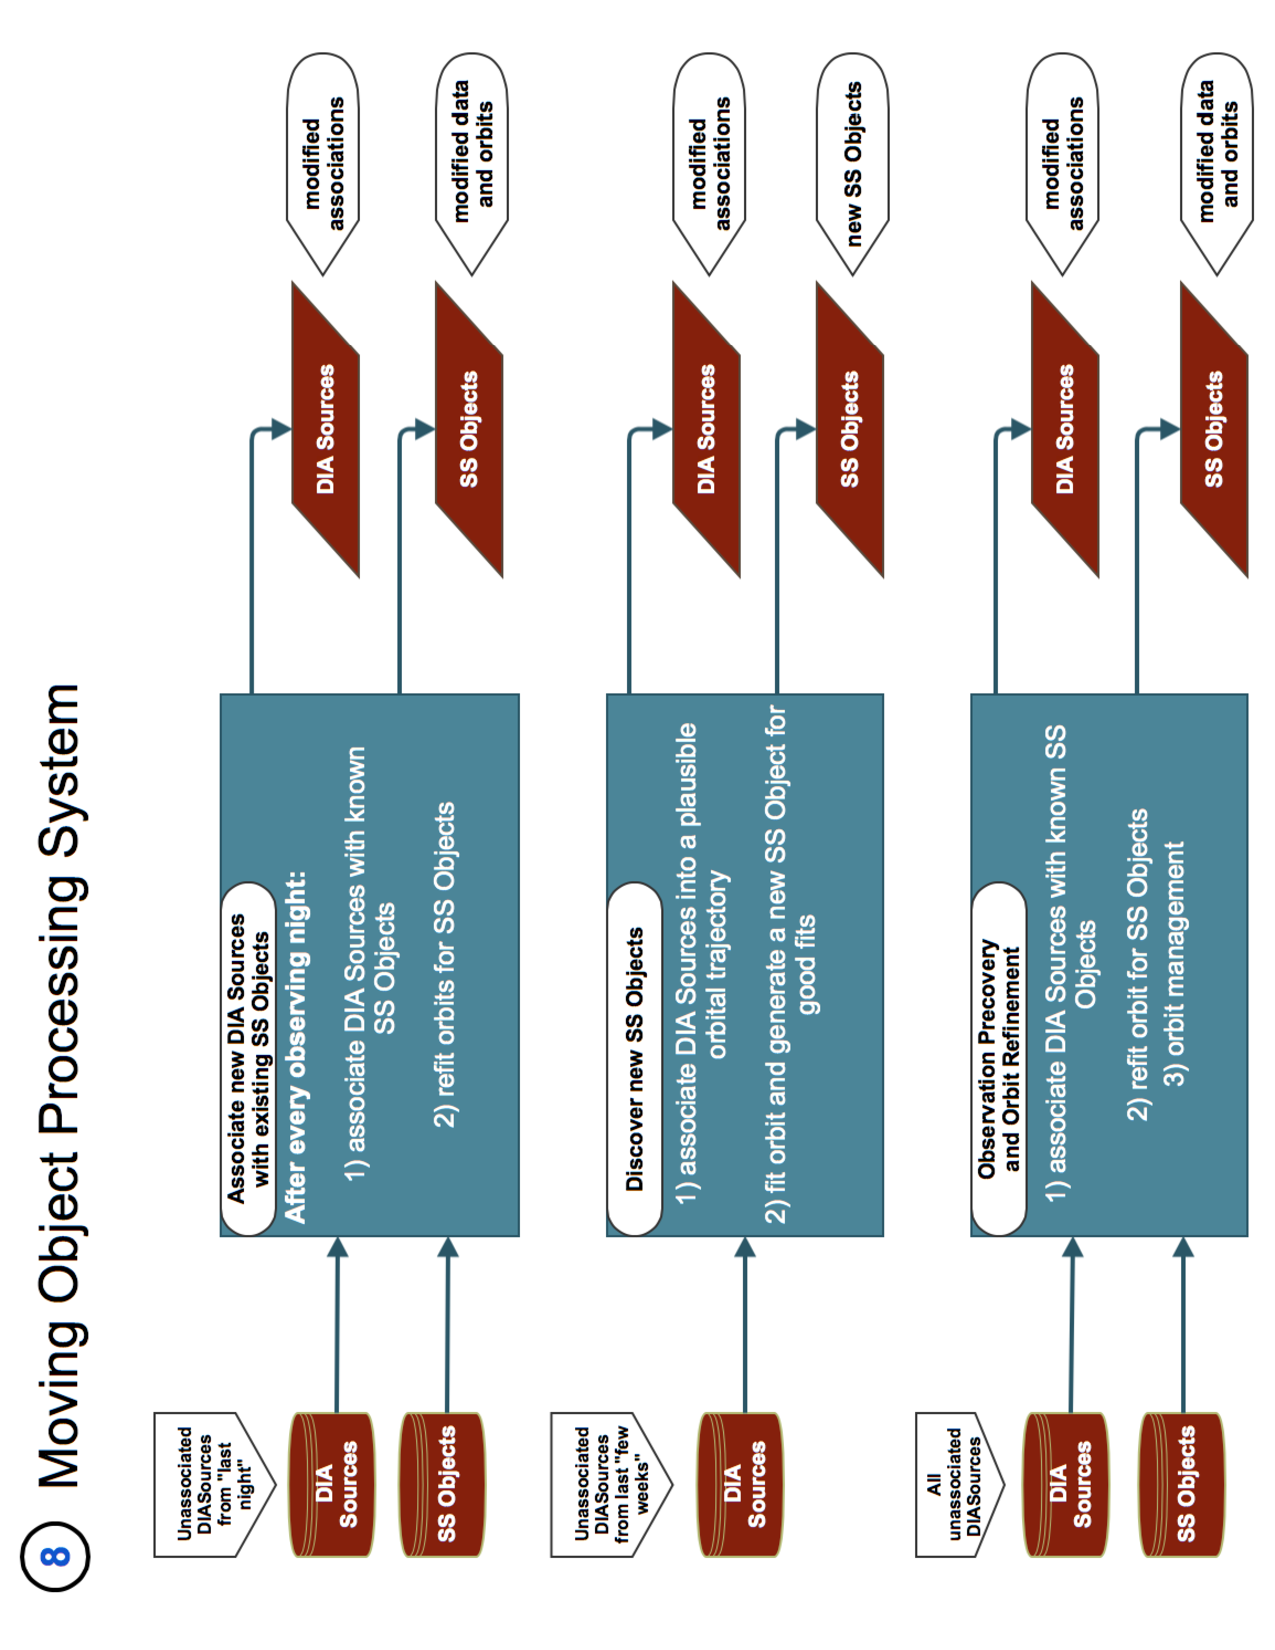
\includegraphics[scale=0.60, angle=270]{MOPS-Level0}
    \vskip -0.1in
    \caption{Illustration of the conceptual algorithm design for the Moving Object Processing System.
   \DIASources are data structures that describe detections of sources in difference images and
   \SSObjects are data structures that describe discovered Solar System objects (see Table~\ref{tab:SSObj}).
\label{fig:Pipe8}}
\end{figure}


\subsection{LSST Level 1 Data Processing}

Level 1 data products are a result of difference image analysis (DIA).
\DIASources are sources detected on difference images with the signal-to-noise ratio $S/N>transSNR$,
with $transSNR$=5.
They represent changes in flux with respect to a deep template. Physically, a \DIASource may be an observation of new astrophysical object that was not present at that position in the template image (for example, an asteroid), or an observation of flux change in an existing source (for example, a variable star). Their flux can be negative (eg., if a source present in the template image reduced its brightness, or moved away). Their shape can be complex (eg., trailed, for a source with proper motion approaching $\sim {\rm deg}/{\rm day}$, or ``dipole-like", if an object's observed position exhibits an offset -- true or apparent -- compared to its position on the template).
Some \DIASources will be caused by background fluctuations; with $transSNR = 5$,
the expected false positive rate is about three per CCD ($\sim 60$ per sq. deg.) for the median seeing,
or of the order 500,000 per typical night.
The expected number of false positives due to background fluctuations is a very strong function
of adopted $transSNR$: a change of $transSNR$ by 0.5
results in a variation of an order of magnitude, and a change of $transSNR$ by unity changes the number of false
positives by about two orders of magnitude.

Clusters of \DIASources detected on visits taken at different times are associated with either a \DIAObject or an \SSObject, to represent the underlying astrophysical phenomenon. The association can be made in two different ways: by assuming the underlying phenomenon is an object within the Solar System moving on an orbit around the Sun\footnote{LSST pipelines will not fit for motion around other Solar System bodies; eg., identifying new satellites of Jupiter is left to the community.}, or by assuming it to be distant enough to only exhibit small parallactic and proper motion\footnote{Where ``small'' is small enough to unambiguously positionally associate together individual apparitions of the object.}. The latter type of association is performed during difference image analysis right after the image has been acquired. The former is done at daytime by \code{MOPS}, unless the \DIASource is an apparition of an already known \SSObject. In that case, it will be flagged as such during difference image analysis. At the end of the difference image analysis of each visit, LSST will issue time domain event alerts for all
newly detected \DIASources\footnote{For observations on the Ecliptic near the opposition Solar System objects will dominate the \DIASource counts and (until they're recognized as such) overwhelm the explosive transient signal. It will therefore be advantageous to quickly identify the majority of Solar System objects early in the survey.}.

\subsubsection{Nightly Difference Image Processing}

The following is a high-level description of steps which will occur during regular {\em nightly}
difference image analysis:
\begin{enumerate}
\item A visit is acquired and reduced to a single {\em visit image} (cosmic ray rejection, instrumental signature removal\footnote{Eg., subtraction of bias and dark frames, flat fielding, bad pixel/column interpolation, etc.}, etc.).
\item The visit image is differenced against the appropriate template and \DIASources are detected and
their properties measured.
\item The flux and shape\footnote{The ``shape'' in this context consists of weighted 2$^{\rm nd}$ moments
of the intensity distribution, as well as fits to a trailed source model and a dipole model.} of the DIASource are measured on the difference image. PSF photometry is performed on the visit image at the position of the \DIASource to obtain a measure of the total flux.
\item The Level 1 database is searched for a \DIAObject or an \SSObject with which to positionally associate the newly discovered \DIASource\footnote{The association algorithm will guarantee that a \DIASource is associated with not more than one existing \DIAObject or \SSObject. The algorithm will take into account the parallax and proper (or Keplerian) motions, as well as the errors in estimated positions of \DIAObject, \SSObject, and \DIASource, to find the maximally likely match. Multiple \DIASources in the same visit will not be matched to the same \DIAObject.}. If no match is found, a new \DIAObject is created and the observed \DIASource is associated to it.
\item If the \DIASource has been associated with an \SSObject (a known Solar System object), it will be flagged as such and an alert will be issued. Further processing will occur in daytime (see \S\ref{sec:ssProcessing} below).
\item Otherwise, the associated \DIAObject measurements will be updated with new data
collected during previous 12 months. All affected columns will be recomputed, including proper motions, centroids, light curves, etc.
\item The \DR\footnote{\DR is a database resulting from annual data release processing.} is searched for \Objects positionally close to the \DIAObject, returning the three nearest stars and three nearest galaxies. The IDs of these nearest-neighbor \Objects are recorded in the \DIAObject record and provided in the issued event alert.
\item An alert is issued that includes the \DIASource ID, the \SSObject ID or \DIAObject ID, and the associated science content (centroid, fluxes, low-order lightcurve moments, periods, etc.), including the full light curves.
\item For all \DIAObjects overlapping the field of view, including those that have an associated
new \DIASource from this visit, forced photometry will be performed on difference image (point source photometry only).
No alerts will be issued for these \DIASources.
\item Within 24 hours of discovery, {\em precovery} PSF forced photometry will be performed on any difference image overlapping the position of new \DIAObjects taken within the past 30 days, and added to the database. Alerts will not be issued with precovery photometry information.
\end{enumerate}

In addition to the processing described above, a smaller sample of sources detected on difference images {\em below} the nominal $transSNR = \transSNR$ threshold will be measured and stored, in order to enable monitoring of difference image analysis quality.

Also, the system will have the ability to measure and alert on a limited\footnote{It will be sized for no less than $\sim 10\%$ of average \DIASource per visit rate.} number of sources detected below the nominal threshold for which additional criteria are satisfied. For example, a $transSNR = 3$ source detection near a gravitational keyhole\footnote{
A gravitational keyhole is a region of space where Earth's gravity would modify the orbit of a passing asteroid
such that the asteroid would collide with the Earth in the future.}
may be highly significant in assessing the danger posed by a potentially hazardous asteroid.
The initial set of criteria will be defined by the start of LSST operations.

\subsubsection{Solar System Object Processing \label{sec:ssProcessing}}

The following will occur during regular Solar System object processing in daytime\footnote{Note that there {\em is no strict bound on when daytime Solar System processing must finish}, just that, averaged over some reasonable timescale (eg., a month), a night's worth of observing is processed within 24 hours. Nights rich in moving objects may take longer to process, while nights with less will finish more quickly. In other words, the system requirement is on {\em throughput}, not latency.}, after a night of observing (see Figure~\ref{fig:Pipe8}):
\begin{enumerate}
\item The orbits and physical properties of all \SSObjects re-observed on the previous night are recomputed. External orbit catalogs (or observations) are also used to improve orbit estimates. Updated data are entered to the \SSObjects table.
\item All \DIASources detected on the previous night, that have {\em not} been matched at a high confidence level to a known \Object,
\DIAObject, \SSObject, or an artifact, are analyzed for potential pairs, forming {\em tracklets}.
\item The collection of tracklets collected over the past 30 days is searched for subsets forming {\em tracks} consistent with being on the same Keplerian orbit around the Sun.
\item For those that are, an orbit is fitted and a new \SSObject table entry created. \DIASource records are updated to point to the new \SSObject record. \DIAObjects ``orphaned'' by this unlinking are deleted.\footnote{Some \DIAObjects may only be left with forced photometry measurements at their location (since all \DIAObjects are force-photometered on previous and subsequent visits);  these will be kept but flagged as such.}.
\item Precovery linking is attempted for all \SSObjects whose orbits were updated in this process. Where successful, \SSObjects (orbits) are recomputed as needed.
\end{enumerate}


\subsubsection{Level 1 Catalogs}
\label{sec:level1db}

The described alert processing design relies on the ``living'' \DB that contains the objects and sources detected on difference images. At the very least\footnote{It will also contain exposure and visit metadata, MOPS-specific tables, etc.}, this database will have tables of \DIASources, \DIAObjects, and \SSObjects, populated in the course of nightly and daily difference image and Solar System object processing\footnote{The latter is also colloquially known as {\em DayMOPS}.}. As these get updated and added to, their updated contents becomes visible (query-able) immediately\footnote{No later than the moment of issuance of any event alert that may refer to it.}.

Table~\ref{tab:SSObj}  presents the {\em conceptual schema} for the \SSObject table (it conveys {\em what} data
will be recorded in each table, rather than the details of {\em how}).
Columns whose type is an array will likely be expanded to one table column per element of the array
once this schema is translated to SQL\footnote{The SQL realization of this schema can be browsed at \url{http://ls.st/8g4}}. In addition, the table presented here is normalized (i.e., it contains no redundant
information with other tables in Level 1 database). For example, since the band of observation can be found
by joining a \DIASource table to the table with exposure metadata, there's no column named {\tt band} in the \DIASource table. In the as-built database, the views presented to the users will be appropriately denormalized
for ease of use.

\subsubsection{\SSObject Table}

\begin{center}
\label{tab:SSObj}
\begin{longtable}{p{3cm}p{2cm}p{2cm}p{5cm}}
%\caption[\SSObject Table]{\SSObject Table} \\

\hline \multicolumn{1}{c}{\bf Name} & \multicolumn{1}{c}{\bf Type} & \multicolumn{1}{c}{\bf Unit} & \multicolumn{1}{c}{\bf Description} \\ \hline
\endhead

\hline \multicolumn{4}{r}{{\em Continued on next page}} \\
\endfoot

\hline\hline
\endlastfoot

ssObjectId & uint64 & ~ & Unique identifier. \\

oe & double[7] & various & Osculating orbital elements at epoch ($q$, $e$, $i$, $\Omega$, $\omega$, $M_0$, epoch). \\

oeCov & double[21] & various & Covariance matrix for \texttt{oe}. \\

arc & float & days & Arc of observation. \\

orbFitLnL & float & ~ & Natural log of the likelihood of the orbital elements fit. \\

orbFitChi2 & float & ~ & $\chi^2$ statistic of the orbital elements fit. \\

orbFitNdata & int & ~ & The number of data points (observations) used to fit the orbital elements. \\

MOID & float[2] & AU & Minimum orbit intersection distances\footnote{\url{http://www2.lowell.edu/users/elgb/moid.html}} \\

moidLon & double[2] & degrees & MOID longitudes. \\

H & float[6] & mag & Mean absolute magnitude, per band (Muinonen et al. 2010 magnitude-phase system). \\

${\rm G_1}$ & float[6] & mag & $G_1$ slope parameter, per band (Muinonen et al. 2010 magnitude-phase system). \\

${\rm G_2}$ & float[6] & mag & $G_2$ slope parameter, per band (Muinonen et al. 2010 magnitude-phase system). \\

hErr & float[6] & mag & Uncertainty of H estimate.\\

g1Err & float[6] & mag & Uncertainty of $G_1$ estimate. \\

g2Err & float[6] & mag & Uncertainty of $G_2$ estimate. \\

flags & bit[64] & bit & Various useful flags. \\ \hline

\end{longtable}
\end{center}

The $G_1$ and $G_2$ parameters for the large majority of asteroids will not be well constrained until later in the survey. LSST may decide not to fit for it at all over the first few DRs and add it later in Operations, or provide two-parameter $G_{12}$ fits. Alternatively, they may be fitted using strong priors on slopes poorly constrained by the data. The design of the data management system is insensitive to this decision, making it possible to postpone it to Commissioning to ensure it follows the standard community practice at that time.
The LSST database will provide functions to compute the phase (Sun-Asteroid-Earth) angle $\alpha$ for every observation, as well as the reduced, $H(\alpha)$, and absolute, $H$, asteroid magnitudes in LSST bands.
 




\bibliography{neo_capabilities}
\end{document}


To Do:

- ask Lori Allen to be coauthor (and if there are others from her team) 
- ask Tim Axelrod and Jonathan Myers (others from old days?) 

Lynne's new NEO runs: cumulative completeness for H<22 objects: 
Run                              3p/30  |3p/15|    SNR3   SNR0   singlePair  singleDet     Modification
astro_lsst_01_1014       76.1      72.6        79.1    94.4       88.8           92.0        12 deg Ecliptic + WFD, 60sec
astro_lsst_01_1015       79.2      74.8        81.7    96.4       90.3           93.0        15 deg Ecliptic + WFD, 60sec
astro_lsst_01_1016       80.0      77.5        83.1    95.6       88.9           92.1        NEO baseline
astro_lsst_01_1017       80.8      77.8        83.3    95.3       90.1           93.1        EB + 30s, gri
lucy_1001                      76.5      73.7        79.9    95.3       88.8           92.1        15 deg Ecliptic (ri, 60 sec), NES gz  




astro_lsst_01_1015:
- the best (but only about half of WFD visits due to 60 sec exposures) 
- how about 20 deg band around the Ecliptic? Going from 12 to 15 has a
    big impact.
- 3 pairs in 30 days at SNR=4 should be similar in completeness to 3
    pairs in 15 days at SNR=3, but more doable 


Run                              3p/30  |3p/15|    SNR3   SNR0   singlePair  singleDet     Modification
astro_lsst_01_1015       79.2      74.8        81.7    96.4       90.3           93.0        15 deg Ecliptic + WFD, 60sec

- at the bright end (H<20), C for single detection and single pair
   saturates at ~99.4%; this shows that 12-year survey is long enough
   to get even those objects that can ``hide behind the Sun'' 
- 3 pairs in 15 nights with SNR=0 results in C=96.4%; this shows that 
   the impact of finite cadence on completeness for *large* objects is 
   only 3.0%
- 3 pairs in 15 nights with SNR=5 gives C=75%, which compared to 
   a single detection with SNR=5 and C=93% represents a loss of 18%;
   therefore, the impact of cadence on *small* objects is much larger 
   than for large objects; going from a single detection to 3 pairs in
   15 nights is equivalent to losing 2 mag of depth! 
- 3 pairs in 15 nights with SNR=5 crosses C=90% at H~20.5; data 
   deeper by 1.5 mag would bring H<22 completeness to 90% (or we'd
   need to go to SNR=1.3); but to go deeper by 1.5 mag, the exposure 
   time needs to be 16 times longer!! 
- going from 15 nights to 30 nights boosts C by 4.4%; this is
   equivalent to about 0.3 mag deeper data and 1.2 mag of ``missing''
   depth; in this case, the exposure time would have to be ``only'' 9
   times longer to reach C=90% for H<22. 
   
So, reaching C=90% is becoming more and more hopeless. My last 
desperate traces of hope are: 
- we could look at the median brightness of (say) H=22 objects vs.
   ecliptic latitude (and perhaps solar elongation to account for
   sweet spots) and adjust exposure time as a function of latitude 
   (we know that the faintest H=22 detections are close to the
   Ecliptic)
- if the required band width is much less than 15 deg, we would 
   perhaps have enough observing time budget to really go with 5-10
   minutes long exposures. Of course, we'd have to keep them down
   to 1 min or so and shift-and-coadd multiple exposures for a grid
   of possible motions, which would be a major impact on DM 
- we could look at H~22 objects which we missed with 3 pairs in 15
   nights, but which we did *not* miss with ``single detection'' and
   ask what were their SNRs when they were in the FOV but didn't 
   have SNR>5. And where they were on the sky. This sounds like 
   something for Joachim to look at. 
- NASA says ``we'd be happy with even C=80%"  :) 


- 75% of the PHAs: Ivezic & Jones, 2014 (AAS)


TODO from May 29 reading: 
- ref to Chesley & JPL, find his simulations plan
- in Introduction, add info about counts of transients from my AAS
time-domain talk, also refer to Ridgway paper
- 



10 km/s at 100 Lunar Distances is:
384,000 km * ang. speed (radian/s)  = 10 km/s 
ang. speed = 5.4 arcsec / sec  = 5.4 * 3600 * 24 arcsec / day   = 5.4*24 ~ 100 deg/day 
5.4 arcsec/sec * 30 sec ~ 3 arcmin trail! 